In questo primo esperimento si vuole dimensionare, costruire e studiare un amplificatore in classe A con specchio di corrente. Il circuito è rappresentato in Figura \ref{fig:Circuit1} ed è composto da tre blocchi principali:
\begin{itemize}\label{ch:Spiegazione1}
    \item Il primo stadio a sinistra è un buffer, connesso a una rete $RC$ ($R_1$ e $C_1$), che ha lo scopo di filtrare la componente continua del segnale $V_{in}$ (che – una volta amplificata – potrebbe danneggiare l’altoparlante).
    \item Il secondo amplificatore operazionale è connesso in configurazione invertente, e serve a controllare il volume. Il volume massimo è limitato dalla presenza della resistenza $R_2$.
    \item Il terzo stadio (stadio di uscita) è un amplificatore in classe A, alimentato da uno specchio di corrente. I due transistor dello specchio sono bipolari di potenza e – per ottenere prestazioni ottimali – dovrebbero avere caratteristiche simili tra loro. 
\end{itemize}
Sono stati utilizzati i seguenti componenti:
\begin{itemize}
    \item $Q_1,Q_2,Q_3$: transistor NPN di potenza con dissipatore, codice TIP41CG
    \item Integrato operazionale a doppia uscita \textit{Rail to Rail}, codice MCP6002
    \item $C_1=220\text{ nF}$, film condensatore di accoppiamento
    \item $R_1=220\text{ k}\Omega, 0.25\text{ W}$ resistenza di ingresso
    \item $R_2$ resistenza limitazione volume da calcolare, $0.25\text{ W}$
    \item $R_{var}$ potenziometro di regolazione volume da $10k\Omega$ logaritmico
    \item $R_L=8\text{ }\Omega,2\text{ W}$ resistenza di carico
    \item $R_S$ resistenza specchio di corrente da calcolare, 2 W
    \item Altoparlante $8\text{ }\Omega,0.2\text{ W}$ codice AS05008PR-2-R
\end{itemize}
\begin{figure}[H]
    \centering
    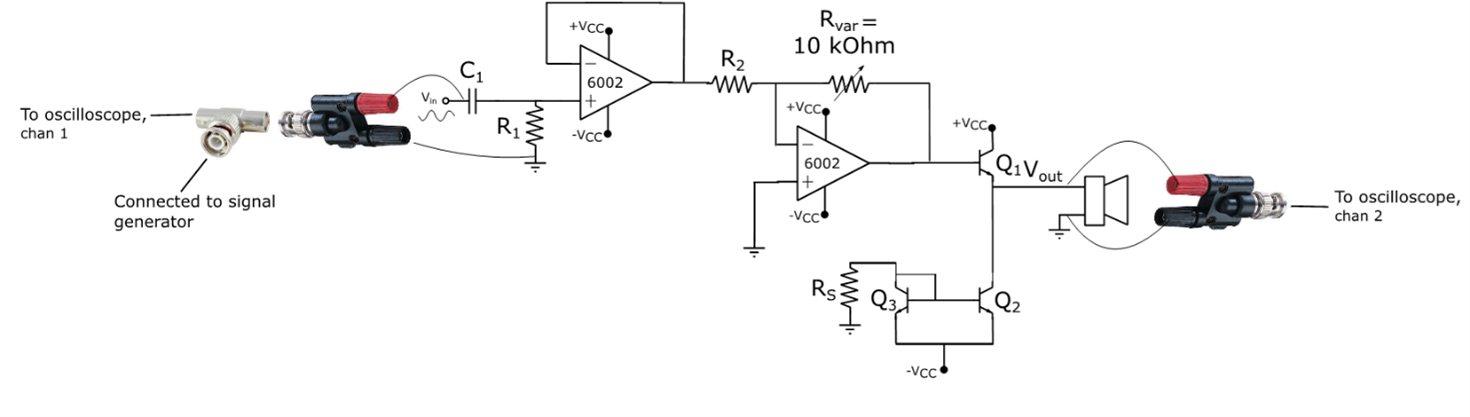
\includegraphics[width=\linewidth]{images/Circuit1.png}
    \caption{schema circuito}
    \label{fig:Circuit1}
\end{figure}
Il circuito è alimentato dalla tensione duale: $\pm V_{CC}=\pm 3V$. Siccome si è a conoscenza che durante l'esperienza i BJT e le resistenze di carico raggiungono temperature elevate, sono stati utilizzati i dissipatori per i transistor bipolari ed è stata prestata particolare attenzione a non toccare tali componenti.\\\\
I pinout dell'integrato MCP6002 sono stati ricavati dal datasheet, riportati in Figura \ref{fig:MCP6002}
\begin{figure}[H]
    \centering
    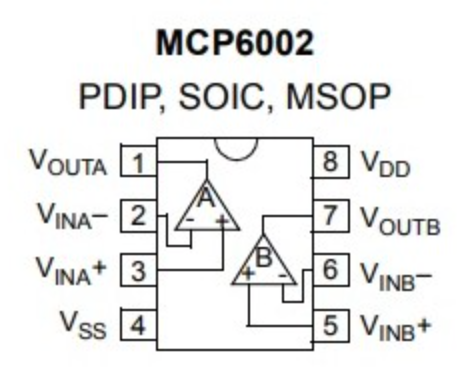
\includegraphics[width=0.2\linewidth]{images/MCP6002.png}
    \caption{Layout dell'integrato MCP6002 }
    \label{fig:MCP6002}
\end{figure}
\subsection{Dimensionamento del circuito - prelab}\label{ch:Prelab1}
Considerato lo specchio di corrente in Figura \ref{fig:CurrentMirror1}. Per prima cosa è stato calcolato il valore della resistenza $R_S$ in modo da garantire una corrente sul carico $(R_L=8\text{ }\Omega)$ pari a $0.3\text{ A}$ anche quando il transistore $Q_1$ è spento. Per determinare tale valore è stata utilizzata la (\ref{eq:Mirror})
\begin{equation}\label{eq:Mirror}
    I=\frac{V_{CC}-V_{BE,3}}{R_S}\implies R_S=3.33\text{ }\Omega
\end{equation}
\begin{figure}[H]
    \centering
    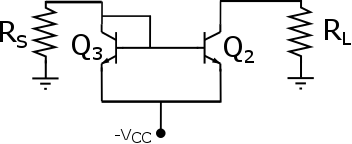
\includegraphics[width=0.5\linewidth]{images/CurrentMirror1.png}
    \caption{Schema circuito dello specchio di corrente}
    \label{fig:CurrentMirror1}
\end{figure}
\noindent Data la disponibilità del laboratorio si è poi scelto di utilizzare una resistenza da $8\text{ }\Omega,2\text{ W}$.\\\\
La resistenza $R_2$ è utilizzata per limitare il volume massimo del circuito ed evitare il surriscaldamento dei transistor. Il suo valore è stato determinato per limitare il guadagno dello stadio invertente ($V_A/V_F$) al valore massimo di 26.0 dB, come imposto dalle specifiche di progetto.
\begin{equation}
    (A_v)_{\text{dB}} = 20\log_{10}{A_v}\quad\text{e}\quad A_v = -\frac{R_{var}}{R_2}
\end{equation}
Da cui abbiamo ricavato il valore di $R_2$ che risulta pari a $501.25\text{ }\Omega$, in laboratorio è stata utilizzata una resistenza da $500\text{ }\Omega$.
\subsection{Analisi in frequenza del circuito - prelab}
Infine è stata è stata calcolata la frequenza di taglio del filtro RC in ingresso.
\begin{equation}
    \omega_C=\frac{1}{\tau}=\frac{1}{R_1C_1}=20.66\quad[\text{rad/s}]
\end{equation}
Il diagramma di Bode della funzione di trasferimento $V_F/V_{in}$ è riportato in Figura \ref{fig:Bode1}.
\begin{figure}[H]
    \centering
    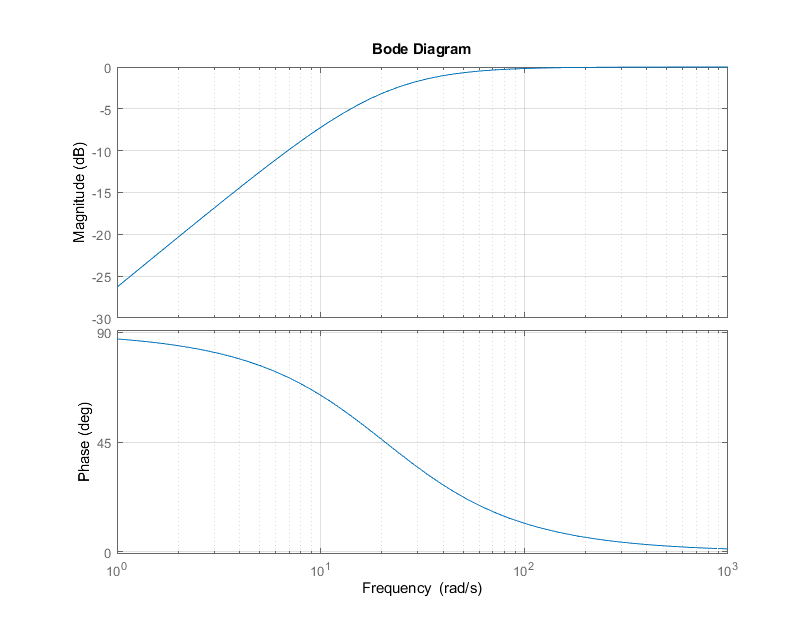
\includegraphics[width=0.7\linewidth]{images/Bode1.png}
    \caption{Diagramma di Bode}
    \label{fig:Bode1}
\end{figure}
\subsection{Risultati laboratorio: prima parte}
Dopo aver montato lo specchio di corrente (Figura \ref{fig:CurrentMirror1}) sulla breadboard, lo si è polarizzato a $-V_{CC}=-3\text{ V}$ e abbiamo misurato con il multimetro la corrente sulle resistenze $R_S$ e $R_L$
\begin{equation*}
    I_{R_S}=0.28\text{ mA}\quad I_{R_L}=0.27\text{ mA}
\end{equation*}
Si può riscontrare una minima differenza fra i due valori di corrente, data dalle tolleranze tra i componenti.
\clearpage
\subsection{Risultati laboratorio: seconda parte}
Per questa parte è stato scollegato lo specchio di corrente per evitare l'inutile riscaldamento dei transistor durante le misure. Abbiamo quindi montato il filtro e il preamplificatore in Figura \ref{fig:PreAmp1}
\begin{figure}[H]
    \centering
    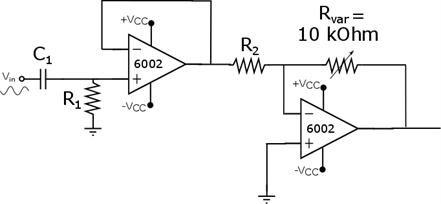
\includegraphics[width=0.7\linewidth]{images/PreAmp1.png}
    \caption{Schema circuito filtro e preamplificatore}
    \label{fig:PreAmp1}
\end{figure}
In seguito è stato collegato il connettore a "T" BNC all'uscita del generatore; una terminazione all'ingresso del circuito  $V_{in}$ e l'altra estremità al canale 1 dell'oscilloscopio. Infine l'uscita dell'amplificatore invertente al canale 2 dell'oscilloscopio. Come si vede dai collegamenti in Figura \ref{fig:PreAmpCircuit1}
\begin{figure}[H]
    \centering
    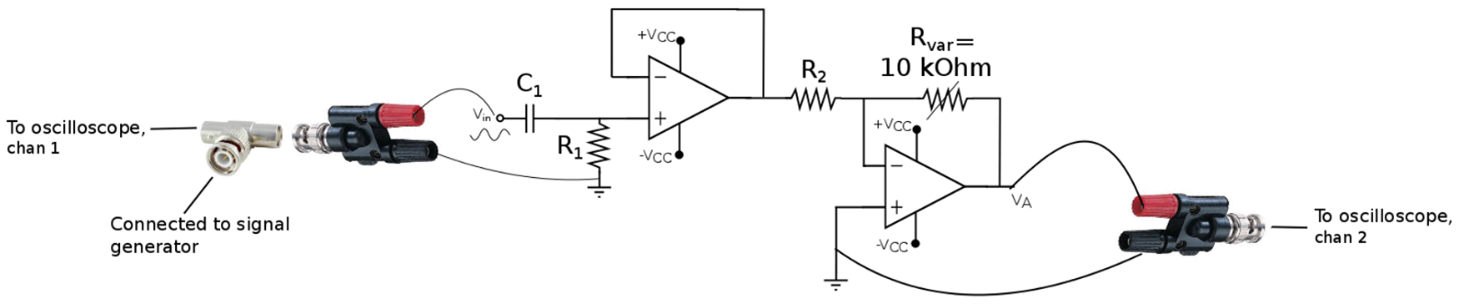
\includegraphics[width=\linewidth]{images/PreAmpCircuit1.png}
    \caption{Schema di collegamento della strumentazione}
    \label{fig:PreAmpCircuit1}
\end{figure}
\noindent Abbiamo impostato il generatore di funzioni per fornire in ingresso al circuito il segnale:
\begin{itemize}
    \item Forma d'onda: sinusoidale
    \item Frequenza: variabile tra 1 Hz e 1000 Hz
    \item Ampiezza: $100\text{ mV}$ picco-picco
\end{itemize}
Il potenziometro $R_{var}$ è stato regolato in modo di avere il massimo guadagno, che corrisponde ad avere il potenziometro a $10\text{ k}\Omega$. Quindi stata fornita l'alimentazione $\pm V_{cc}=\pm3\text{ V}$ all'integrato e abbiamo misurato con l'oscilloscopio il segnale di uscita del circuito alle varie frequenze di ingresso. Riportiamo in Tabella \ref{tab:Ris1} le misure effettuate e il guadagno$\left|V_A/V_{in}\right|_{dB}$ del circuito.
\begin{table}[H]
    \centering
    \begin{tabular}{|c|c|c|}
        \hline
        Frequenza (Hz)&$V_{A_{pp}}$&$\left|V_A/V_{in}\right|_{dB}$\\\hline\hline
        1&610mV&15.119\\\hline
        3&1.34V&21.954\\\hline
        5&1.68V&23.919\\\hline
        10&1.9V&24.987\\\hline
        30&1.99V&25.389\\\hline
        50&1.99V&25.389\\\hline
        100&1.99V&25.389\\\hline
        300&2V&25.433\\\hline
        500&2.01V&25.476\\\hline
        1000&2.03V&25.562\\\hline
    \end{tabular}
    \caption{Misura del guadagno $\left|V_A/V_{in}\right|_{dB}$}
    \label{tab:Ris1}
\end{table}
Il diagramma di Bode in Figura \ref{fig:Bode2} è tracciato a partire dai dati in Tabella \ref{tab:Ris1} è stato confrontato con l'andamento teorico calcolato nella Sezione \ref{ch:Prelab1}, si nota che il valore $R_2$ scelto permette effettivamente di limitare il guadagno del circuito a $26.0\text{ dB}$. Inoltre il diagramma in Figura \ref{fig:Bode1} è stato tracciato considerando il solo filtro, con relativo buffer e non lo stadio di amplificazione; questo giustifica il discostamento dal diagramma i Bode in Figura \ref{fig:Bode2}.
\begin{figure}[H]
    \centering
    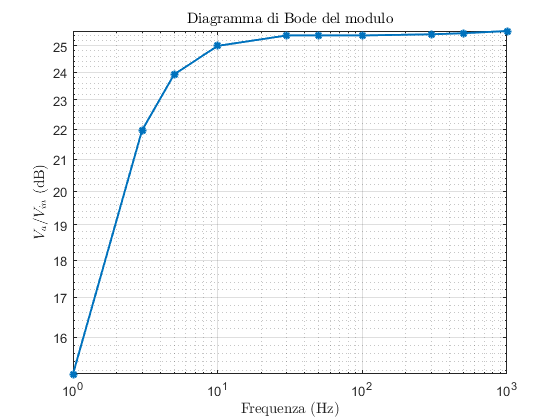
\includegraphics[width=0.8\linewidth]{images/Bode2.png}
    \caption{Diagramma di Bode dai dati della Tabella \ref{tab:Ris1}}
    \label{fig:Bode2}
\end{figure}
\clearpage
\subsection{Risultati laboratorio: terza parte}
È stato collegato lo stadio in classe A al filtro, come indicato in figura \ref{fig:Circuit1}. Il circuito è stato connesso all'alimentazione, al generatore di segnale e all'altoparlante.\\\\
Al circuito è stato applicato in ingresso il segnale con le seguente caratteristiche
\begin{itemize}
    \item Forma d'onda: sinusoidale
    \item Frequenza: 330 Hz (nota Mi)
    \item Ampiezza: $100\text{ mV}$ picco-picco
\end{itemize}
Abbiamo regolato il potenziometro del volume $R_{var}$ in modo da raggiungere un'ampiezza di $1\text{ } V_{pp}$ sul segnale di uscita.\\\\
Abbiamo impostato l'oscilloscopio per misurare il segnale di ingresso $V_{in}$ e di uscita $V_{out}$. Riportiamo in Figura \ref{fig:scope_4} la schermata dell'oscilloscopio con i due segnali
\begin{figure}[H]
    \centering
    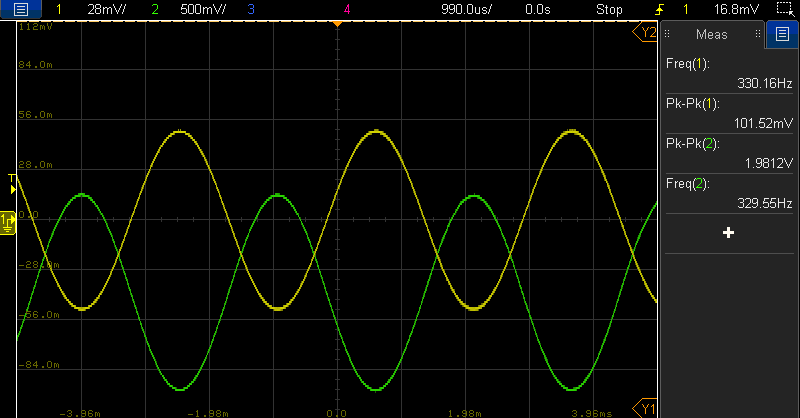
\includegraphics[width=0.7\linewidth]{images/scope_4.png}
    \caption{Segnale in ingresso e in uscita dall'amplificatore}
    \label{fig:scope_4}
\end{figure}
Non siamo riusciti ad arrivare a $1\text{ } V_{pp}$ in quanto le componenti non ce lo permettevano. Infatti pur portando il potenziometro a fondo scala il segnale di uscita $V_{out}$ è rimasto a $1.9812\text{ } V_{pp}$.\\\\
Abbiamo poi misurato i segnali $V_{out} \text{ e } V_{B,Q1}$. Abbiamo riportato in Figura \ref{fig:scope_5} la schermata di acquisizione in modalità "normale" e in Figura \ref{fig:scope_6} in modalità XY con l'intento misurare la differenza tra i due segnali.
\begin{figure}[H]
    \centering
    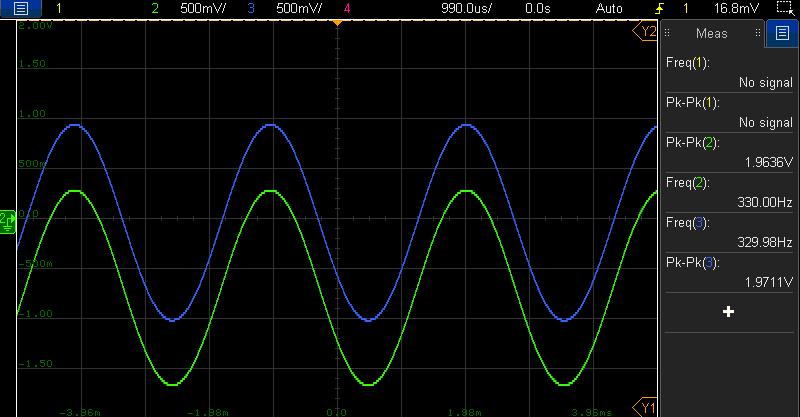
\includegraphics[width=0.7\linewidth]{images/scope_5.png}
    \caption{Segnali $V_{out} \text{ e } V_{B,Q1}$}
    \label{fig:scope_5}
\end{figure}
\begin{figure}[H]
    \centering
    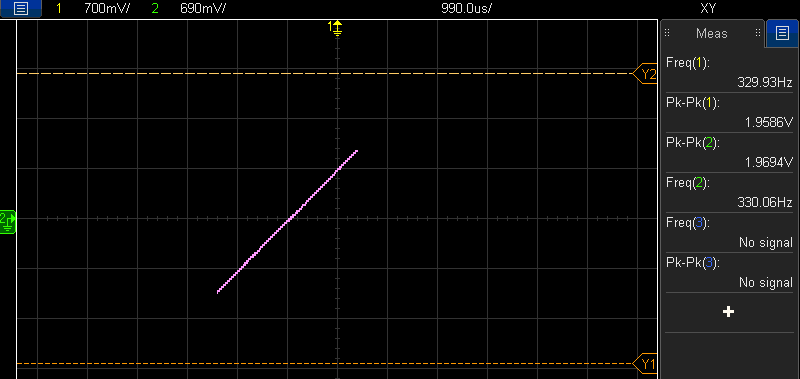
\includegraphics[width=0.7\linewidth]{images/scope_6.png}
    \caption{Segnali $V_{out} \text{ e } V_{B,Q1}$ in modalità XY}
    \label{fig:scope_6}
\end{figure}
Dalla Figura \ref{fig:scope_6} possiamo ben apprezzare che la differenza tra i due segnali è costante in tutto il periodo, infatti in modalità XY (Figura \ref{fig:scope_6}) abbiamo ottenuto una retta. Come si poteva facilmente prevedere la differenza è pari a $V_{be}$.
\subsection{Risultati laboratorio: ultima parte}
Infine si è stimata l'efficienza del circuito in queste condizioni
\begin{equation}
    \eta=\frac{\text{load power}}{\text{supply power}}=\frac{1}{2}\frac{V_{OP}^2}{R_L}\frac{1}{VV_{CC}}=\frac{1}{4}\frac{V_{OP}^2}{IR_LV_{CC}}=\dots
\end{equation}
Si può apprezzare come l'amplificatore in classe A sia praticamente esente da distorsioni ma soffre di una efficienza bassissima, questo si è notato anche durante gli esperimenti in quanto i componenti del finale di potenza si sono particolarmente surriscaldati.\\\\
Si conclude l'esperienza connettendo un dispositivo con jack a 3.5mm all'uscita del circuito, tuttavia l'altoparlante non funzionava correttamente quindi si è deciso di usare una resistenza da 8$\Omega$. Si utilizzata tale resistenza anche nelle esperienze successive in sostituzione dell'altoparlante.